\chapter{The project}
\label{chapter2}


\section{The Nowcasting.com trial}
\label{chapter2_section1}

To design inovative investment strategies, CFM is continuously testing alternative datasets and new data providers. In 2020, CFM benefited from a trial proposed by the company Now-casting.com. Founded by former ECB economist Lucrezia Reichlin, Now-Casting.com is an online service delivering high frequency, short-term forecasts for the world’s major economies, in real time. These forecasts (or ``nowcasts'') are generated by a dynamic factor model initially developed by \cite{Giannone2008}. Specifically, the model uses a large dataset of several dozens of monthly macroeconomic data to predict the lower frequency, quarterly real GDP growth rate. The services of Now-casting.com cover a wide range of countries and geographic areas such as the United States, the Euro Area, Japan, Germany, Italy, Spain or the United Kingdom. The econometric methodologies they use permit not only to predict the growth rate of real GDP, but also to forecast any monthly feature involved in the model. These features include key macroeconomic and financial variables like industrial production, business sales, consumer prices, house constructions, federal funds rates, or mortgage rates.

If these predictions are accurate, the dataset certainly carries useful information for investment decisions, and CFM might find added value in using the service. During the internship, the first task thus consisted in investigating the dataset, exploring a number of countries and features, and comparing the predictions with the ground truth. This resulted in a brief report (the complete report can be found in Appendix \ref{appendix1}).

Overall the conclusions were mixed, both regarding the accuracy of the predictions and the model capacity to improve its predictions while new information obtains. Certain countries like the Euro area seemed to produce fairly good GDP nowcasts, the latter effectively improving while more information was added to the model. Other countries like Italy displayed really poor performance, with prediction errors switching back and forth until the release date of GDP. This is illustrated in Figure \ref{fig_c2_s1_1}.

\begin{figure} [H]

\centering

\begin{subfigure}[t]{0.43\textwidth}

	\centering

	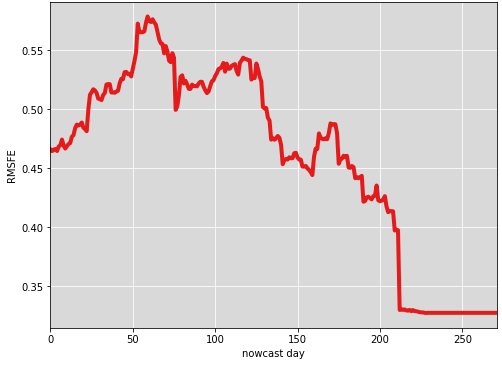
\includegraphics[width=\linewidth]{images/rmse_gdp_ea.png}

	\caption{Euro Area}
\end{subfigure} 	\hspace{1cm}
\begin{subfigure}[t]{0.4\textwidth}

	\centering

	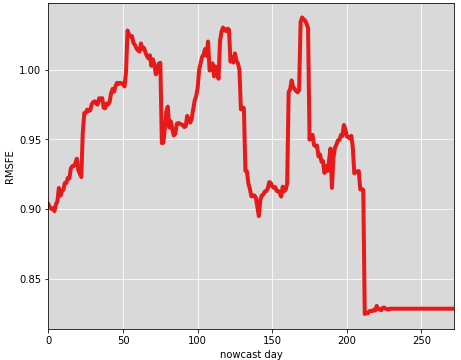
\includegraphics[width=\linewidth]{images/rmse_gdp_it.png}

	\caption{Italy}
\end{subfigure}

\caption{Average RMSE of Nowcasting.com on predictions for GDP growth}

\label{fig_c2_s1_1}
\vspace{-3mm}
\end{figure}

For the other features, the conclusions were overall similar. The predictions ranged from fair (Business confidence index for the Euro area) to absurd, with RMSE continuously increasing as more information becomes available (new car registrations in the Euro Area). This is demonstrated by Figure \ref{fig_c2_s1_2}.

\begin{figure} [H]

	\centering

	\begin{subfigure}[t]{0.43\textwidth}

		\centering

		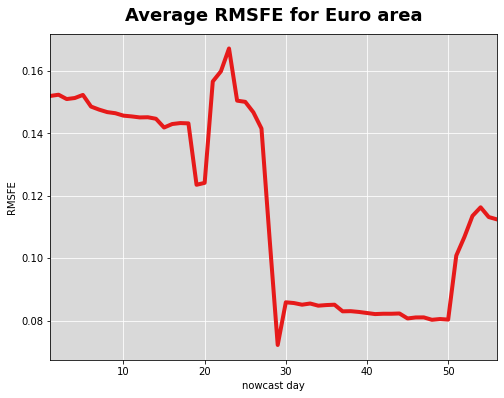
\includegraphics[width=\linewidth]{images/rmse_business_ea.png}

		\caption{Business confidence index}
	\end{subfigure} 	\hspace{1cm}
	\begin{subfigure}[t]{0.43\textwidth}

		\centering

		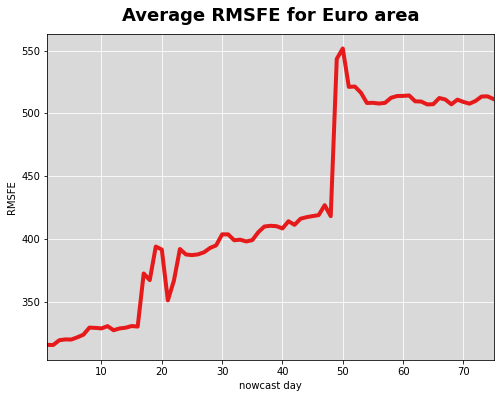
\includegraphics[width=\linewidth]{images/rmse_car_ea.png}

		\caption{New car registrations}
	\end{subfigure}

	\caption{Average RMSE of Nowcasting.com on feature predictions}

	\label{fig_c2_s1_2}
\vspace{-3mm}
\end{figure}

These mediocre performances were not fully convincing. This proved especially true for the United States, which yet represents the main country for macro-financial decision making. The significant price of the service then led to a simple consideration: could it be possible to replicate internally the dynamic factor model used by Now-casting.com, and achieve performances that prove equal - or better - than the ones they propose? As a first step, the United States sounded like a natural candidate since is one of the key countries for global macroeconomic developments, and because long series of data are easily and publicly available.
